\documentclass{beamer}
\usepackage{multicol}
\usepackage{subcaption}
\usepackage{float}

\usetheme{Copenhagen}
\defbeamertemplate*{footline}{mysplit theme}
{%
	\leavevmode%
	\hbox{\begin{beamercolorbox}[wd=.2\paperwidth,ht=2.5ex,dp=1.125ex,leftskip=.3cm plus1fill,rightskip=.3cm]{author in head/foot}%
			\usebeamerfont{author in head/foot}\insertshortauthor
		\end{beamercolorbox}%
		\begin{beamercolorbox}[wd=.7\paperwidth,ht=2.5ex,dp=1.125ex,leftskip=.3cm]{title in head/foot}%
			\usebeamerfont{title in head/foot}\insertshorttitle
	\end{beamercolorbox}
	\begin{beamercolorbox}[wd=.1\paperwidth,ht=2.5ex,dp=1.125ex,leftskip=.4cm,rightskip=.3cm]{title in head/foot}
		\insertframenumber/\inserttotalframenumber
	\end{beamercolorbox}
	}
	\vskip0pt%
}

\setbeamertemplate{navigation symbols}{}
\setbeamertemplate{bibliography item}{[\theenumiv]}
\setbeamertemplate{frametitle continuation}[from second]
%\setbeamertemplate{footline}{
%	\hspace*{0.1cm}
%	\text{short title}
%	\hspace{1cm}
%	\insertshortauthor
%	\hspace{3.5cm}
%	\insertsectionhead
%	\hfill
%	\insertframenumber
%	/
%	\inserttotalframenumber
%	\hspace{0.1cm}
%}

\title[Implementació d'un sistema criptogràfic en sistemes de comptadors intel·ligents]{\textbf{Implementació d'un sistema criptogràfic per l'enviament del consum en sistemes de comptadors intel·ligents}}
\author{Oriol Alàs Cercós}

\institute[Universitat de Lleida]{
	\normalsize Francesc Sebé\\
	\texttt{francesc.sebe@udl.cat} \newline\newline
	Criptografia i Grafs\\
	Universitat de Lleida
}
\date{15 de juliol del 2021}

\begin{document}
\begin{frame}
\centering

\Large\textbf{Implementació d'un sistema criptogràfic per l'enviament del consum en sistemes de comptadors intel·ligents}
\vspace{0.5cm}\\

\normalsize
Oriol Alàs Cercós
\\
\texttt{oriol.alas@udl.cat}
\vspace{0.5cm}\\
Francesc Sebé Feixas
\\
\texttt{francesc.sebe@udl.cat}
\small \vspace{0.3cm}\\
Criptografia i Grafs
\\
Universitat de Lleida
\vspace{0.5cm}\\
15 de juliol del 2021
\end{frame}
\begin{frame}
	\frametitle{Taula de continguts}
	    \begin{columns}[onlytextwidth,T]
		\begin{column}{.45\textwidth}
			\tableofcontents[sections=1-2]
		\end{column}
		\begin{column}{.45\textwidth}
			\tableofcontents[sections=3-5]
		\end{column}
	\end{columns}
\end{frame}

\section{Introducció}
\subsection{Plantejament}
\begin{frame}{Introducció}
	\begin{figure}
		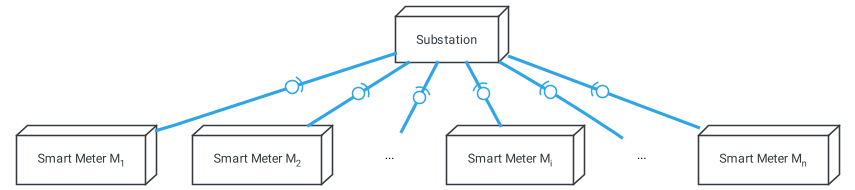
\includegraphics[width=10cm]{../umls/network.png}
	\end{figure}
\end{frame}
\subsection{Objectius}
\begin{frame}{Introducció}{Objectius}
	Objectius:
	\begin{itemize}
		\item Estudiar la solució proposada.
		\item Posar en context el xifratge homomòrfic i el criptosistema asimètric ElGamal.
		\item Implementar un client que simuli un comptador intel·ligent.
		\item Implementar un servidor que simuli una subestació d'una comunitat de comptadors.
		\item Realitzar un estudi dels costs del protocol.
	\end{itemize}
\end{frame}
%\section{Estat de l'art}
%\subsection{Xifratge simètric i asimètric}
%\subsection{Xifratge homomòrfic}

\section{Propostes}
\subsection{Tipus de propostes}
\begin{frame}
	\frametitle{Tipus de propostes}
	\begin{itemize}
		\item \alert<1-2>{Propostes pertorbatives}\\
		\only<2>{
			\vspace{1em}
			Afegir un soroll a les lectures per tal de
transmetre un resultat diferencial.
			\[\sum_{i=1}^{N} m_i \approx \sum_{i=1}^{N} (m_i + x_i)\]}
		\item \uncover<3->{\alert<3-4>{Propostes anònimes}}
		\only<4>{
			\begin{block}{Objectiu}
				Anonimitzar les dades del consum per tal de no poder determinar fàcilment una llar.
			\end{block}
			\begin{itemize}
				\item High-Frequency ID
				\item Low-Frequency ID
			\end{itemize}
		}
		\item \uncover<5->{\alert<5->{Propostes agregatives}}\\
		\only<6>{
			\vspace{1em}
			Els comptadors s’agreguen en comunitats per tal de sumar les seves
lectures abans de transmetre-les a la subestació.
			\vspace{0.5em}
			\begin{itemize}
				\item Xifratge homomòrfic.
				\begin{itemize}
					\item Intercanvi de claus.
					\item Distribuïdor de claus.
				\end{itemize}
			\end{itemize}
		}
	\end{itemize}
\end{frame}

\subsection{Proposta \cite{busom}}
\begin{frame}{Proposta \cite{busom}}
\begin{itemize}
	\item Proposta agregativa.
	\item ElGamal aprofitant homorfisme sobre la multiplicació.
	\begin{itemize}
		\item Es pot usar tant en $\mathbb{Z}_p$ com $E(\mathbb{Z}_p)$.
	\end{itemize}
	\item Fases:
	\begin{itemize}
		\item Configuració de claus.\\Usa intercanvi de claus en lloc d'un distribuïdor de claus.
		\item Transmissió del consum.
	\end{itemize}
\end{itemize}
\end{frame}

\begin{frame}{Proposta \cite{busom}}{Configuració de claus}
	\begin{multicols}{2}
		
		\begin{figure}
			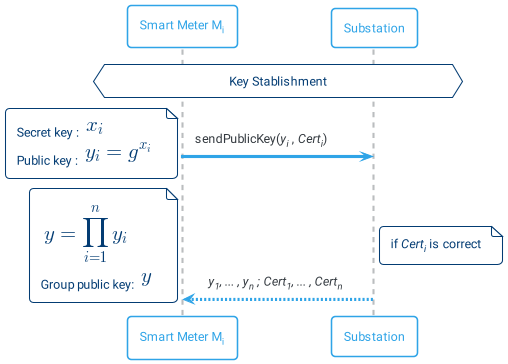
\includegraphics[width=14em]{images/busom2.png}
		\end{figure}
	\newpage
	\begin{itemize}
		\item $M_i$ té la clau secreta $x_i \in \mathbb{Z}_q^* $ i la clau pública $y_i = g^{x_i}$
		\item Intercanvi de claus Diffie-Hellman: $y = g^{\sum_{i=1}^{n} x_i}$
		
	\end{itemize}
	\end{multicols}
\end{frame}

\begin{frame}{Proposta \cite{busom}}{Transmissió del consum}
		\begin{multicols}{2}
		
		\begin{figure}
			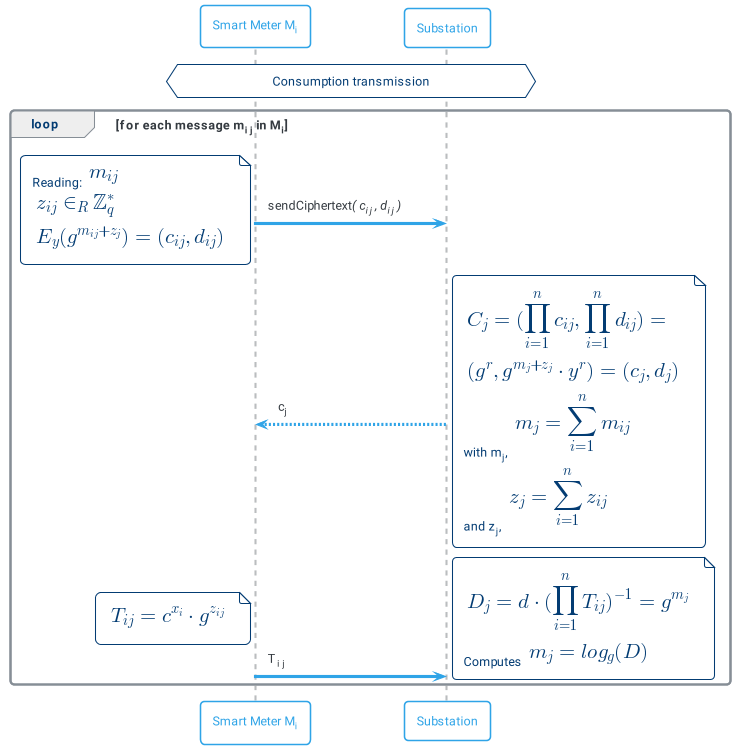
\includegraphics[width=14em]{images/busom3.png}
		\end{figure}
		\newpage
		\begin{itemize}
%			\tiny
			\only<1-2>{\item \small Cada comptador $M_i$ genera un valor aleatori i envia \normalsize $E_y(g^{m_i+z_i}) = (c_i, d_i)$}
			\only<2>{\item \small La subestació agrega tots els xifrats:
			\begin{align*}
				C &= (\prod_{i=1}^{n} c_i, \ \prod_{i=1}^{n} d_i)\\
				&= (g^r, \ y^r \cdot g ^{\sum_{i=1}^{n} m_i} \cdot g^z)\\
				&= (g^r, \ y^r \cdot g ^{m + z})\\
				&= (c, d)
			\end{align*}}
			\only<3>{\item Cada comptador $M_i$ rep $c$ i envia la seva contribució perquè la subestació realitzi el logaritme discret.}
			\only<3>{\[T_i = c^{x_i} \cdot g^{z_i}\]}
			\only<4>{\item La subestació agrega les contribucions de manera que:
			\begin{align*}
				T &= \prod_{i=1}^{n} T_i = c^x \cdot g^z = g^{r \cdot x + z}\\
				&= y^r \cdot g^z, \qquad x = \sum_{i=1}^{n} x_i	
			\end{align*}}
		\only<4>{\item Troba $g^m$ realitzant \[g^m = d \cdot T^{-1}\]}
		\only<5>{\item Finalment, realitza el logaritme discret per tal de trobar $m$:
		\[m = log_g(D)\]}
		\end{itemize}
	\end{multicols}
\end{frame}

\subsection{Proposta \cite{recsi}}
\begin{frame}{Proposta \cite{recsi}}
	\begin{itemize}
		\item Proposta agregativa.
		\item Fases:
		\begin{itemize}
			\item Configuració de claus.
			\\Usa intercanvi de claus \alert{amb una restricció} en lloc d'un distribuïdor de claus.
			\[k_{Sst} = - \sum_i^{N} k_{m_i}\]
			\item Transmissió del consum.
		\end{itemize}
	\end{itemize}
%	\uncover<2>{\begin{block}{Restricció}
%			La clau de la subestació serà l'element simètric de la suma de claus dels comptadors.
%	\end{block}}
\end{frame}

\begin{frame}{Proposta \cite{recsi}}{Configuració de claus}
	\begin{multicols}{2}
		
		\begin{figure}
			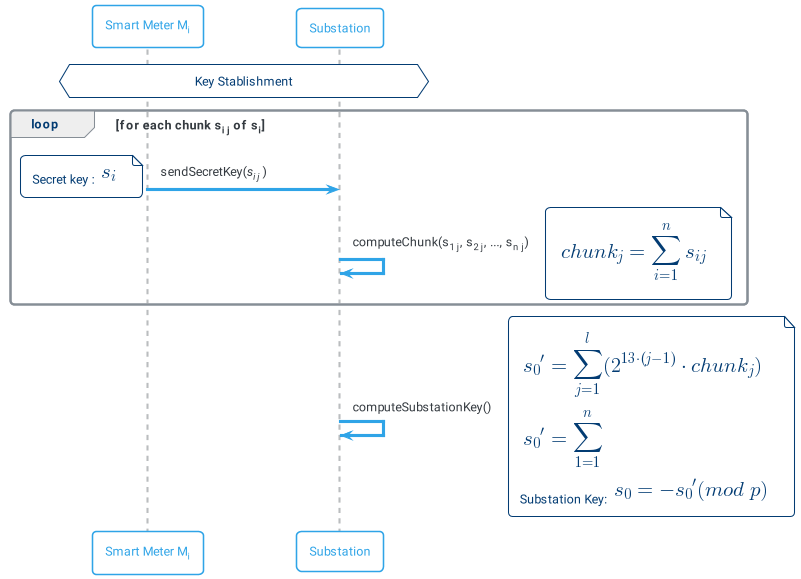
\includegraphics[width=15em]{images/recsi1.png}
		\end{figure}
		\newpage
		\begin{itemize}
			\only<1-2>{\item  Cada comptador $M_i$ genera el seu secret $s_i$.}
			\only<2-3>{\item  Aquesta és dividida en $l$ fragments de, com a màxim, 13 bits:
			\[s_i = (s_{il} || ... || s_{i2} || s_{i1})\]}
			\only<3>{\item  Per tal de saber només la suma dels fragments, s'usa el protocol \cite{busom}.}
			\only<4-5>{\item En cada iteració, la subestació obtindrà:
			\[\sum_{i=1}^{n}s_{ij}\]}
			\only<5-6>{\item La subestació concatenarà els diferents resultats:
			\[s_0^{'} = \sum_{j=1}^{l} \Big( 2^{13 \cdot (j - 1)} \cdot \sum_{i=1}^{n} s_{ij} \Big)\]}
			\only<6->{Finalment, calcularà l'element simètric de $s_0^{'}$:
			\[s_0\ =\ - s_0^{'} \quad (mod \ p)\]}
		\end{itemize}
	\end{multicols}
\end{frame}

\begin{frame}{Proposta \cite{recsi}}{Transmissió del consum}
	\begin{multicols}{2}
		
		\begin{figure}
			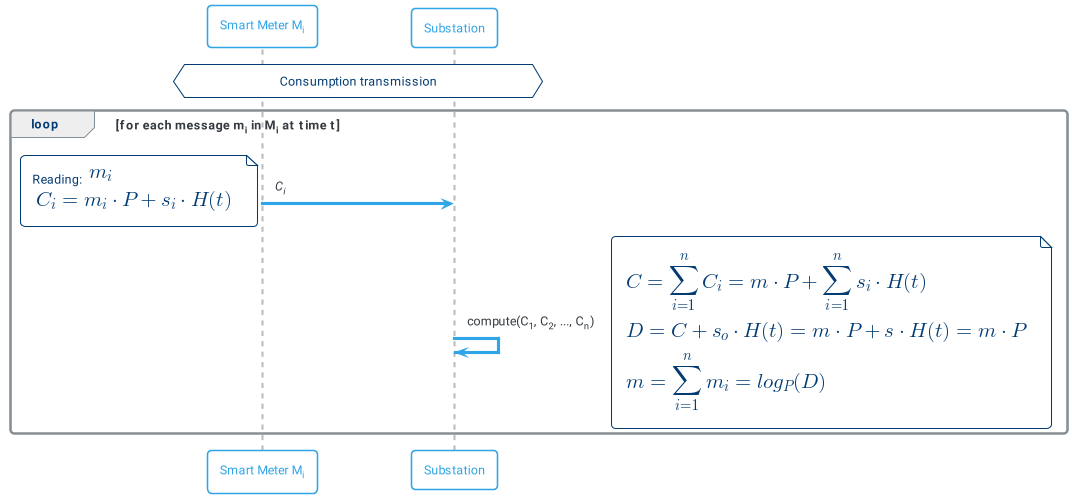
\includegraphics[width=15em]{images/recsi2.png}
		\end{figure}
		\newpage
		\begin{itemize}
			\only<1>{\item Cada comptador $M_i$ transmet de manera xifrada:
			\[C_i = m_i \cdot P + s_i + H(t)\]
			}
			\only<2>{\item La subestació suma els xifrats obtenint un punt resultant C:
			\[C = \sum_{i=1}^{n}c_i = m \cdot P + \sum_{i=1}^{n}s_i \cdot H(t)\]	
			\[= m \cdot P + s_0^{'}\cdot H(t)\]}
			\only<3>{\item La subestació eliminarà el soroll provocat per les claus secretes:
			\begin{align*}
			D &= C + s_0 \cdot H(t)\\
			&= m \cdot P + (s_0^{'} + s_0) \cdot H(t)\\
			& = m \cdot P
			\end{align*}
			\[m = \sum_{i=1}^{n} = log_P(D)\]
			}
		\end{itemize}
	\end{multicols}
\end{frame}

\section{Disseny de la implementació}
\begin{frame}{Disseny de la implementació}{Especificacions}
	\begin{itemize}
		\item Arquitectura client-servidor.
		\item \texttt{CigLib}
		\item \texttt{Java 8}
		\item \texttt{Apache Maven 3.6.3}
	\end{itemize}
\end{frame}
\begin{frame}{Disseny de la implementació}
Arquitectura del projecte:
\begin{itemize}
	\alert<1>{
	\item \texttt{crypt}.
	\item \texttt{busom}.
	\item \texttt{recsi}. \pause}
	\alert<2>{
	\item \texttt{connection}.
	\item \texttt{consumption}. \pause}
	\alert<3>{
	\item \texttt{main}.}
\end{itemize}
\end{frame}
\subsection{Criptografia}
\begin{frame}
	\begin{figure}
		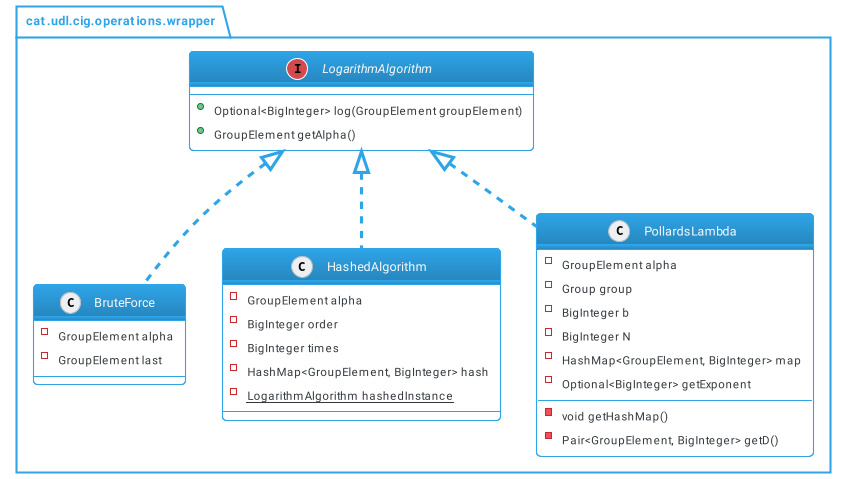
\includegraphics[width=28em]{images/log}
	\end{figure}
\end{frame}
\subsection{Patró Màquina-Estat}
\begin{frame}{Disseny de la implementació}{Patró Màquina-Estat}
	Propietats del patró:
	\begin{itemize}
		\item Implementar la lògica d'estats i transicions.
		\item Aporta rigidesa al sistema.
		\item Dificulta l'asincronia.
	\end{itemize}
\end{frame}
\begin{frame}
	\begin{figure}
		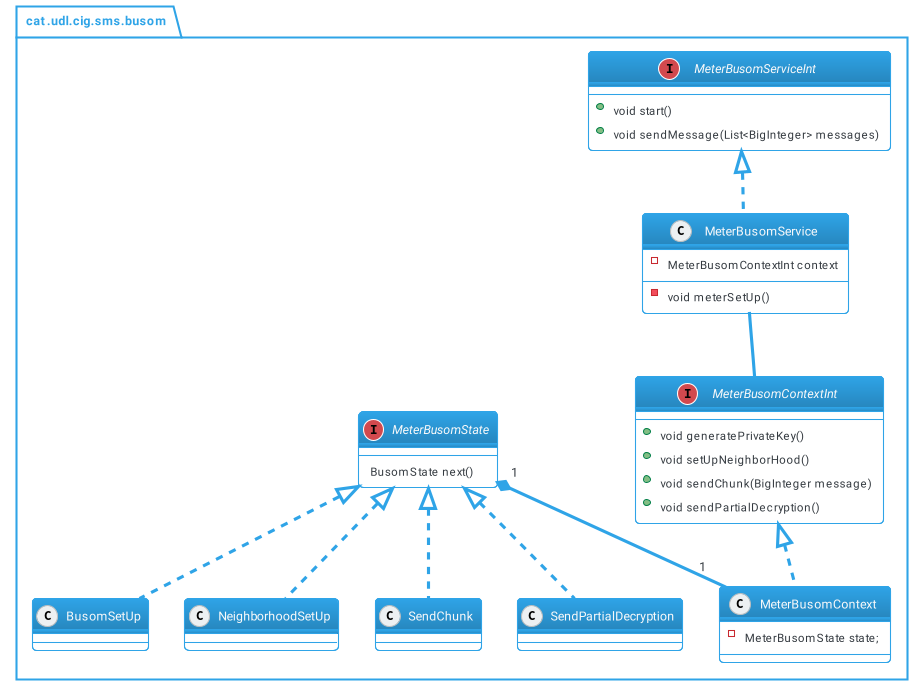
\includegraphics[width=28em]{images/busomprot}
	\end{figure}
\end{frame}

\section{Anàlisi de costos}
\begin{frame}{Anàlisi de costos}
	\begin{itemize}
		\item \alert<1>{Algorismes de computació del logaritme discret} \pause
		\item \alert<2>{Comparació entre \cite{busom} i \cite{recsi}} \pause
		\item \alert<3>{Simulació usant dades reals}
		\only<3>{
		\begin{figure}
		\begin{multicols}{2}
			\begin{figure}
				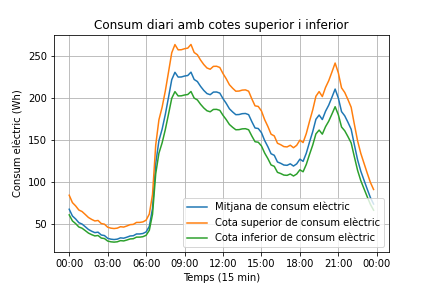
\includegraphics[width=13em]{images/consumption2.png}
			\end{figure}
			\newpage
			\begin{figure}
				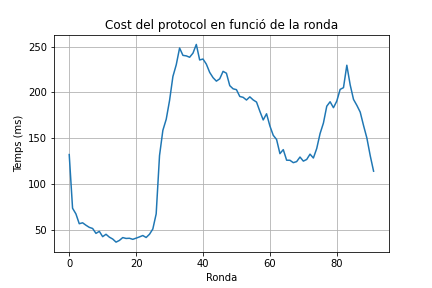
\includegraphics[width=13em]{images/consumption.png}
			\end{figure}
		\end{multicols}
		\caption{Comparació entre la gràfica de consum i gràfica del cost en temps segons la ronda.}
		\end{figure}}
	\end{itemize}
\end{frame}
\subsection{Logaritme discret}

\begin{frame}{Anàlisi de costos}{Logaritme discret}
	\begin{multicols}{2}
	\begin{figure}
		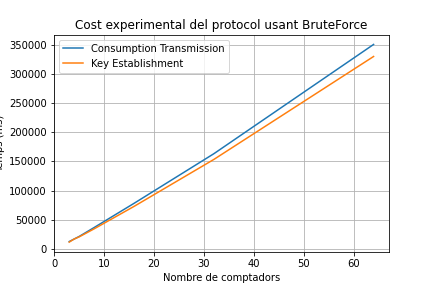
\includegraphics[width=14em]{images/brute.png}
	\end{figure}
	\newpage
	\begin{figure}
		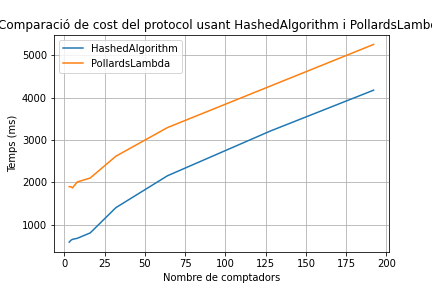
\includegraphics[width=14em]{images/comp.png}
	\end{figure}
\end{multicols}
\end{frame}

\begin{frame}{Anàlisi de costos}{Logaritme discret}
	\begin{multicols}{2}
		\begin{figure}
			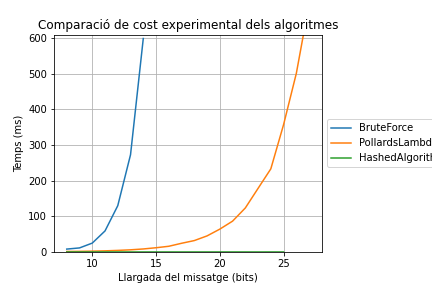
\includegraphics[width=14em]{images/algoritmes-cost.png}
		\end{figure}
		\newpage
		\begin{figure}
			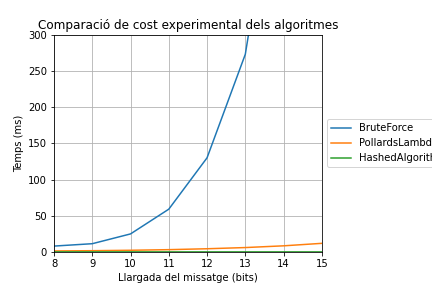
\includegraphics[width=14em]{images/algoritmes-cost2.png}
		\end{figure}
	\end{multicols}
\end{frame}

\subsection{Comparació entre propostes}
\begin{frame}{Anàlisi de costos}{Comparació entre propostes}
	\begin{figure}
		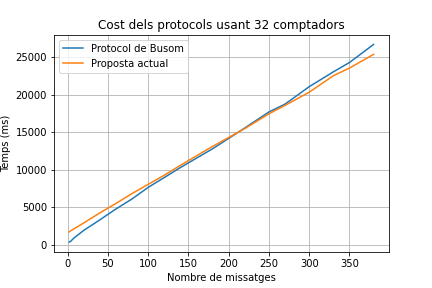
\includegraphics[width=14em]{images/32compt.png}
	\end{figure}
\end{frame}

\begin{frame}
	Es millor usar \cite{busom} si:
	\only<1>{
	\[Cost_1(R) < Cost_2(R)\]
	}
	\only<2>{
	\begin{align*}
		Cost_1(R) &< Cost_2(R)\\
		Cost_{KE_1} + Cost_{CT_1}(R) &<  Cost_{KE_2} + Cost_{CT_2}(R)
	\end{align*}
	}
	\only<3->{
	\begin{align*}
		Cost_1(R) &< Cost_2(R)\\
		Cost_{KE_1} + Cost_{CT_1}(R) &<  \alert<3>{Cost_{1}(|Fragments|)} + Cost_{CT_2}(R)
	\end{align*}
	}
	\only<4->{
	Simplificant el problema, trobem que:
	\alert<4>{\[Cost_{CT_1}(R) = Cost_{CT_2}(R) \cdot k_{\textrm{comunicació}}, \qquad k_{\textrm{comunicació}} \ge 1\]}
	}
	\only<5->{Per tant,}
	\only<5>{
	\[Cost_{KE_1} + \alert{Cost_{CT_2}(R) \cdot k_{\textrm{comunicació}}} \le  Cost_{1}(|Fragments|) + Cost_{CT_2}(R)\]
	}
	\only<6>{\[Cost_{KE_1} <  Cost_{1}(|Fragments|) + \alert{Cost_{CT_2}(R) \cdot (1 - k_{\textrm{comunicació}})}\]}
	\only<7>{
		\[Cost_{KE_1} <  \alert{Cost_{KE_1} + Cost_{CT_1}(|Fragments|)} + Cost_{CT_2}(R) \cdot (1 - k_{\textrm{comunicació}})\]
	}
	\only<8>{
		\[\alert{0} < Cost_{CT_1}(|Fragments|) + Cost_{CT_2}(R) \cdot (1 - k_{\textrm{comunicació}})\]
	}
	\only<9>{\[ |Cost_{CT_2}(R) \cdot (1 - k_{\textrm{comunicació}})| < Cost_{CT_1}(|Fragments|)\]}
\end{frame}
\begin{frame}{Treball futur}
	\begin{itemize}
		\item Seria interessant analitzar els protocols incloent aquesta
		vegada \cite{repair-busom}.
		\item Aprendre nous protocols i aprofitar el codi de l’aplicació i la llibreria per analitzar
		entre altres protocols i veure el seu rendiment.
		\item Aprendre computació quàntica i usar una llibreria per a veure si el protocol actual
		pot tenir algun defecte de seguretat o possible vulnerabilitat en la transmissió de
		claus o lectures.
	\end{itemize}
	
\end{frame}
\begin{frame}[allowframebreaks]
	\frametitle{Referències}
	\tiny{\bibliographystyle{unsrt}}
	\bibliography{references}
\end{frame}
\end{document}